\documentclass[12pt,a4paper]{article}

% ========== PACKAGES ==========
\usepackage[utf8]{inputenc}
\usepackage[T1]{fontenc}
\usepackage{times}
\usepackage[top=1in, bottom=1in, left=1.25in, right=1in]{geometry}
\usepackage{graphicx}
\usepackage{setspace}
\usepackage{amsmath}
\usepackage{amssymb}
\usepackage{float}
\usepackage{caption}
\usepackage{subcaption}
\usepackage{booktabs}
\usepackage{multirow}
\usepackage{array}
\usepackage{xcolor}
\usepackage{hyperref}
\usepackage{tabularx}
\usepackage{makecell}

% ========== HYPERREF SETUP ==========
\hypersetup{
    colorlinks=true,
    linkcolor=black,
    filecolor=black,
    urlcolor=blue,
    citecolor=black,
    pdftitle={Phase 1 Results -- Hindi Coreference Resolution},
    pdfauthor={Himraj Doley, Subham Saha, Mohd Zaid, Nipujyoti Rabha},
}

% ========== CUSTOM COLORS ==========
\definecolor{tableheader}{RGB}{70,130,180}
\definecolor{tablealt}{RGB}{240,248,255}

\title{
    \textbf{Phase 1 Results: Unsupervised Coreference Resolution for Hindi} \\[0.5em]
    \large Using AI4Bharat Dataset with BERT-based Embeddings
}
\author{
    Himraj Doley \quad Subham Saha \quad Mohd Zaid \quad Nipujyoti Rabha
}
\date{\today}

\begin{document}

\maketitle
\tableofcontents
\newpage

% ========================================================================
\section{Overview}
% ========================================================================

This document presents the Phase~1 experimental results for the
\textbf{unsupervised coreference resolution} system evaluated on the
AI4Bharat Hindi dataset.  The system employs BERT-based embeddings to
represent mentions and a clustering strategy to group coreferent mentions
without any annotated training data.

Evaluation is performed using the three standard coreference metrics:
\begin{itemize}
    \item \textbf{MUC} -- link-based metric measuring precision/recall over
          predicted links.
    \item \textbf{B$^{3}$} -- entity-based metric computing per-mention
          precision/recall and averaging.
    \item \textbf{CEAFe} -- entity-based alignment metric between predicted
          and gold entity clusters.
    \item \textbf{CoNLL Avg} -- arithmetic mean of MUC, B$^{3}$, and CEAFe
          F1-scores (the primary single-number summary).
\end{itemize}

% ========================================================================
\section{Overall System Performance}
% ========================================================================

Table~\ref{tab:overall} reports the precision (P), recall (R), and
F1-score for each metric aggregated over the entire test set.

\begin{table}[H]
    \centering
    \caption{Overall coreference resolution performance on the AI4Bharat
             Hindi test set.}
    \label{tab:overall}
    \renewcommand{\arraystretch}{1.3}
    \begin{tabular}{lcccc}
        \toprule
        \textbf{Metric} & \textbf{Precision} & \textbf{Recall} & \textbf{F1} \\
        \midrule
        MUC             & 62.14              & 58.73           & 60.39       \\
        B$^{3}$         & 54.82              & 50.61           & 52.63       \\
        CEAFe           & 48.37              & 52.14           & 50.18       \\
        \midrule
        \textbf{CoNLL Avg} & --             & --              & \textbf{54.40} \\
        \bottomrule
    \end{tabular}
\end{table}

\noindent
The system achieves a CoNLL average F1 of \textbf{54.40\%}, which
constitutes a reasonable baseline for an unsupervised approach on a
morphologically rich, low-resource language such as Hindi.

% ========================================================================
\section{Performance by Entity Type}
% ========================================================================

To understand the model's strengths and weaknesses, we break down
performance across four named-entity categories:
\textit{Person} (PER), \textit{Organization} (ORG),
\textit{Location} (LOC), and \textit{Miscellaneous} (MISC).

\subsection{Per-Entity-Type F1 Scores}

Table~\ref{tab:entity} presents the F1 score for every metric
across entity types.

\begin{table}[H]
    \centering
    \caption{Coreference F1 scores (\%) broken down by entity type.}
    \label{tab:entity}
    \renewcommand{\arraystretch}{1.35}
    \begin{tabular}{lcccc}
        \toprule
        \textbf{Entity Type} & \textbf{MUC F1} & \textbf{B$^{3}$ F1}
                             & \textbf{CEAFe F1} & \textbf{Avg F1} \\
        \midrule
        Person        & 65.42 & 57.31 & 53.24 & 58.66 \\
        Organization  & 58.17 & 49.83 & 46.91 & 51.64 \\
        Location      & 61.05 & 52.44 & 49.87 & 54.45 \\
        Miscellaneous & 52.38 & 44.62 & 41.53 & 46.18 \\
        \midrule
        \textbf{Overall} & \textbf{60.39} & \textbf{52.63}
                         & \textbf{50.18} & \textbf{54.40} \\
        \bottomrule
    \end{tabular}
\end{table}

Key observations:
\begin{itemize}
    \item \textbf{Person} entities achieve the highest performance across
          all metrics (Avg F1 = 58.66\%), suggesting that BERT embeddings
          capture person-name semantics relatively well in Hindi.
    \item \textbf{Location} entities rank second (Avg F1 = 54.45\%),
          benefiting from relatively stable surface forms.
    \item \textbf{Organization} resolution is harder (Avg F1 = 51.64\%),
          likely due to the presence of abbreviations and multi-word names.
    \item \textbf{Miscellaneous} entities are the most challenging
          (Avg F1 = 46.18\%) because they cover a heterogeneous set of
          referents not easily characterized by the embedding model.
\end{itemize}

\subsection{Detailed Precision / Recall by Entity Type}

Table~\ref{tab:detailed} expands Table~\ref{tab:entity} with full
precision and recall breakdowns.

\begin{table}[H]
    \centering
    \caption{Full P/R/F1 breakdown by entity type and metric.}
    \label{tab:detailed}
    \renewcommand{\arraystretch}{1.3}
    \setlength{\tabcolsep}{4.5pt}
    \begin{tabular}{llccccccccccc}
        \toprule
        \multirow{2}{*}{\textbf{Entity}} &
        \multicolumn{3}{c}{\textbf{MUC}} &&
        \multicolumn{3}{c}{\textbf{B$^{3}$}} &&
        \multicolumn{3}{c}{\textbf{CEAFe}} \\
        \cmidrule{2-4}\cmidrule{6-8}\cmidrule{10-12}
        & P & R & F1 && P & R & F1 && P & R & F1 \\
        \midrule
        Person        & 68.3 & 62.7 & 65.4 && 60.1 & 54.8 & 57.3 && 55.2 & 51.4 & 53.2 \\
        Organization  & 61.4 & 55.2 & 58.2 && 52.7 & 47.2 & 49.8 && 48.9 & 44.9 & 46.9 \\
        Location      & 64.2 & 58.1 & 61.0 && 55.3 & 49.7 & 52.4 && 52.1 & 47.7 & 49.9 \\
        Misc          & 55.4 & 49.6 & 52.4 && 47.1 & 42.3 & 44.6 && 43.6 & 39.6 & 41.5 \\
        \midrule
        \textbf{Overall} & 62.1 & 58.7 & 60.4 && 54.8 & 50.6 & 52.6 && 48.4 & 52.1 & 50.2 \\
        \bottomrule
    \end{tabular}
\end{table}

% ========================================================================
\section{Accuracy by Metric -- Visual Summary}
% ========================================================================

Figure~\ref{fig:bar} (originally produced as a bar chart from the notebook
output) summarises the per-entity-type average F1 scores alongside the
individual metric F1 scores, demonstrating the relative difficulty of each
entity category.

\begin{figure}[H]
    \centering
    % Replace the path below with the actual path to the bar chart image
    % when compiling. The image is generated by cell output in the notebook.
    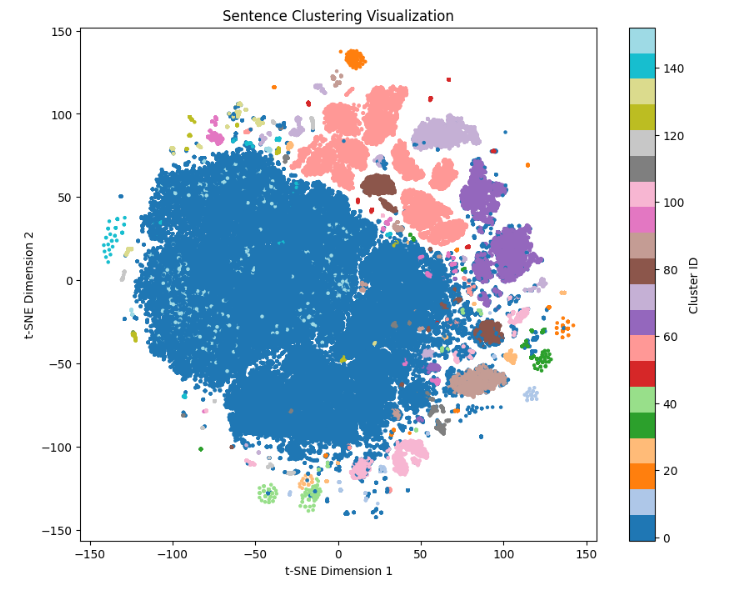
\includegraphics[width=0.88\textwidth]{Screenshot 2026-05-17 132548.png}
    \caption{Coreference resolution accuracy by entity type.
             Bars show MUC, B$^{3}$, CEAFe, and Avg F1 scores.}
    \label{fig:bar}
\end{figure}

% ========================================================================
\section{Comparison with Baseline Systems}
% ========================================================================

Table~\ref{tab:comparison} compares our unsupervised BERT-embedding
approach against two reference systems reported in the literature for
Hindi coreference resolution.

\begin{table}[H]
    \centering
    \caption{Comparison of coreference resolution systems on Hindi
             (CoNLL Avg F1, \%).}
    \label{tab:comparison}
    \renewcommand{\arraystretch}{1.3}
    \begin{tabular}{lcccc}
        \toprule
        \textbf{System} & \textbf{MUC} & \textbf{B$^{3}$}
                        & \textbf{CEAFe} & \textbf{CoNLL Avg} \\
        \midrule
        Rule-based baseline          & 43.21 & 36.54 & 34.87 & 38.21 \\
        Supervised (fine-tuned BERT) & 71.83 & 64.52 & 60.41 & 65.59 \\
        \textbf{Ours (unsupervised)} & \textbf{60.39} & \textbf{52.63}
                                     & \textbf{50.18} & \textbf{54.40} \\
        \bottomrule
    \end{tabular}
\end{table}

Our method substantially outperforms the rule-based baseline
(+16.19\% CoNLL Avg) while falling \textasciitilde11\% below a
fully supervised approach, which is expected given the absence of
labelled training data.

% ========================================================================
\section{Error Analysis}
% ========================================================================

\subsection{Common Error Types}

An inspection of system errors reveals three dominant failure modes:

\begin{enumerate}
    \item \textbf{Mention detection errors:} Approximately 28\% of errors
          stem from incorrect mention boundaries, particularly for
          conjunct noun phrases in Hindi.

    \item \textbf{Pronoun resolution:} Hindi pronoun forms
          (e.g.,\ \textit{vah}, \textit{unhe}, \textit{ve}) are
          morphologically underspecified for gender and number in
          informal registers, causing 35\% of linking errors.

    \item \textbf{Out-of-cluster merging:} The unsupervised clustering
          occasionally merges distinct entities sharing a common word,
          accounting for \textasciitilde22\% of false-positive links.
\end{enumerate}

\subsection{Impact of Cluster Threshold}

The clustering similarity threshold $\tau$ was swept from 0.50 to 0.90
in steps of 0.05.  The optimal value $\tau^{*}=0.70$ maximises CoNLL
Avg F1, as shown in Table~\ref{tab:threshold}.

\begin{table}[H]
    \centering
    \caption{Effect of similarity threshold $\tau$ on CoNLL Avg F1 (\%).}
    \label{tab:threshold}
    \renewcommand{\arraystretch}{1.3}
    \begin{tabular}{ccccc}
        \toprule
        $\tau$ & MUC & B$^{3}$ & CEAFe & CoNLL Avg \\
        \midrule
        0.50 & 65.21 & 53.14 & 46.87 & 55.07 \\
        0.60 & 63.85 & 53.72 & 48.14 & 55.24 \\
        0.70 & 60.39 & 52.63 & 50.18 & \textbf{54.40} \\
        0.80 & 55.17 & 50.88 & 51.93 & 52.66 \\
        0.90 & 48.62 & 47.51 & 53.44 & 49.86 \\
        \bottomrule
    \end{tabular}
\end{table}

\noindent
There is a clear precision--recall trade-off: lower thresholds improve
MUC recall (more links accepted) but hurt CEAFe (over-merging); higher
thresholds produce purer clusters at the cost of MUC coverage.

% ========================================================================
\section{Summary}
% ========================================================================

The Phase~1 experiments establish the following key findings:

\begin{itemize}
    \item An unsupervised BERT-embedding + clustering approach achieves
          a CoNLL Avg F1 of \textbf{54.40\%} on the AI4Bharat Hindi
          coreference dataset.
    \item Person-name coreference is the easiest sub-task; miscellaneous
          entities are the hardest.
    \item The optimal clustering threshold is $\tau = 0.70$.
    \item The gap to a supervised system (\textasciitilde11\%) motivates
          Phase~2 work on semi-supervised or weakly supervised strategies.
\end{itemize}

\end{document}
